%%%%%%%%%%%%%%%%%%%% VIBETEST -- EMNLP 2026 (ARR May cycle) %%%%%%%%%%%%%%%%%
%
% Uses the official ACL style files from
%   https://github.com/acl-org/acl-style-files
% You need: acl.sty, acl_natbib.bst, vibetest.bib, and this file in the same
% directory.
%
% Compile with: pdflatex -> bibtex -> pdflatex -> pdflatex
%
% Submission mode:
%   \usepackage[review]{acl}    % anonymous
%   \usepackage{acl}            % camera-ready
%   \usepackage[preprint]{acl}  % arXiv version
%
%%%%%%%%%%%%%%%%%%%%%%%%%%%%%%%%%%%%%%%%%%%%%%%%%%%%%%%%%%%%%%%%%%%%%%%%%%%%%%%

\documentclass[11pt]{article}

\usepackage[review]{acl}

\usepackage{times}
\usepackage{latexsym}
\usepackage[T1]{fontenc}
\usepackage[utf8]{inputenc}
\usepackage{microtype}
\usepackage{booktabs}
\usepackage{multirow}
\usepackage{array}
\usepackage{amsmath}
\usepackage{amssymb}
\usepackage{graphicx}
\usepackage{xcolor}
\usepackage{url}
\usepackage{tikz}
\usetikzlibrary{arrows.meta,positioning,shapes.geometric}
\usepackage[capitalize,noabbrev]{cleveref}

% Comment marker macros -- colored notes in draft, removed in final.
\newcommand{\todo}[1]{\textcolor{red}{\textbf{[TODO: #1]}}}
\newcommand{\arkan}[1]{\textcolor{blue}{[AK: #1]}}
\newcommand{\adam}[1]{\textcolor{purple}{[AS: #1]}}

\title{Vibetest: Verifying Evidence for LLM-Agent\\Audits of Machine Learning Pipelines}

% Anonymous for review submission -- acl.sty [review] option hides this.
\author{Anonymous ACL submission}

\begin{document}
\maketitle

\begin{abstract}
Repository-level machine learning correctness is difficult to validate because many important requirements are stated only in natural language.
At the same time, LLM agents are increasingly used to inspect and modify real codebases from high-level instructions.
We study whether such agents can reliably audit ML repositories against informal correctness properties, focusing on a key requirement for trust: a reported failure should come with evidence that makes the failure independently verifiable.
We introduce \textbf{Vibetest}, an LLM-agent auditor that evaluates a repository against a natural-language property and returns a \textsc{pass}/\textsc{fail}/\textsc{inconclusive} decision with cited evidence.
We evaluate Vibetest on two ML-pipeline settings: a synthetic controlled benchmark of 75 Kaggle-style notebooks with GPT-5.2-codex-injected bugs and known ground truth, and a real-world audit of 121 public Kaggle notebooks across tabular, text, and image classification.
Vibetest detects many real issues, but its \textsc{fail} evidence precision is moderate: 58.8\% on the synthetic benchmark and 66.1\% in the full real-world audit.
A stricter re-audit of 100 real \textsc{fail}s shows that many unsupported failures share the same structure: the agent treats missing evidence of satisfaction as evidence of violation.
We evaluate a post-hoc LLM evidence verifier that scores whether each \textsc{fail} is justified by the cited evidence.
The current same-backbone verifier is not yet a reliable filter, but the analysis identifies a concrete requirement for future LLM-agent auditors: \textsc{fail} decisions should require evidence of a present-and-violating operation, while absence or unverifiability should be \textsc{inconclusive}.
\end{abstract}

\section{Introduction}

The correctness of repository-scale machine learning systems remains difficult to test.
Many important failures are not local syntax errors or type errors, but violations of high-level intent: training on held-out data, applying augmentation to evaluation splits, reporting metrics on the wrong split, failing to beat a simple baseline, or silently using degenerate preprocessing.
These properties are natural for practitioners to describe in English, but expensive to encode as formal specifications or reusable static checks.

At the same time, software engineering is being reshaped by increasingly capable LLM agents.
Modern agents can inspect repositories, run commands, edit files, and reason over high-level instructions.
Benchmarks such as SWE-bench \citep{jimenez2024swebench} measure whether agents can fix real issues, and repository-level auditing systems such as RepoAudit \citep{guo2025repoaudit} and BugScope \citep{liu2025bugscope} explore whether agents can find bugs.
This raises a natural question for ML code: can an LLM agent validate a repository against a natural-language correctness property without requiring a hand-written formal checker?

The answer depends not only on whether the agent emits the right label, but also on whether it provides verifiable evidence.
For code auditing, a \textsc{fail} verdict is useful only if a user can inspect the cited evidence and confirm that it demonstrates a violation.
This distinction is especially important in ML notebooks.
If a notebook does not run a randomized-label sanity check, that is missing evidence; it does not prove that randomized labels would fail to reduce performance.
If no training-loss plot is logged, that is not evidence that training loss failed to decrease.
In these cases, the right verdict is often \textsc{inconclusive}, not \textsc{fail}.

We study this issue through \textbf{Vibetest}, an LLM-agent auditor for ML pipelines.
Given a repository and a natural-language property, Vibetest operates in a sandboxed copy of the repository, gathers evidence through code inspection and execution, and returns a \textsc{pass}, \textsc{fail}, or \textsc{inconclusive} decision with an evidence report.
Our focus in this paper is not merely agentic testing as a general paradigm, but evidence-based verification of the agent's reported failures.

We evaluate Vibetest in two complementary settings.
First, we construct a controlled synthetic Kaggle benchmark by prompting GPT-5.2-codex to inject known ML-pipeline bugs into clean notebooks.
This gives 75 injected notebooks, 1,125 notebook-property pairs, and ground truth for both precision and recall.
Second, we run Vibetest on 121 real public Kaggle notebooks from Titanic, Disaster Tweets, and Diabetic Retinopathy Detection.
Because the full set of real bugs is unknown, we manually audit all 380 emitted \textsc{fail} verdicts for evidence correctness and perform a stricter 100-case re-audit to validate the rubric.

Our main finding is that many incorrect \textsc{fail} verdicts are not arbitrary.
They follow a single structural pattern: Vibetest emits \textsc{fail} when the cited evidence supports only \textsc{inconclusive}.
Across surface failure modes such as absence-as-failure, best-practices-as-requirements, notebook over-interpretation, and missing-output-as-incorrect-output, the underlying error is the same.
The agent treats the absence of an expected operation as evidence that the operation was performed incorrectly.

Following Adam Stein's proposed verifier direction, we evaluate an additional post-hoc step: an LLM verifier receives the test prompt, Vibetest's reasoning, and the cited evidence, then outputs a score from 0 to 1 indicating whether the evidence supports the \textsc{fail}.
This score lets us plot precision-recall tradeoffs over accepted failures and directly test whether unsupported failures can be pruned.
In the current run, however, the same-backbone verifier is close to chance on synthetic predicted failures and below chance on the strict real re-audit.
This negative result is important: evidence verification is necessary, but a naive verifier built from the same model family can inherit the auditor's evidential blind spots.

\begin{figure*}[t]
  \centering
  \resizebox{0.96\linewidth}{!}{%
  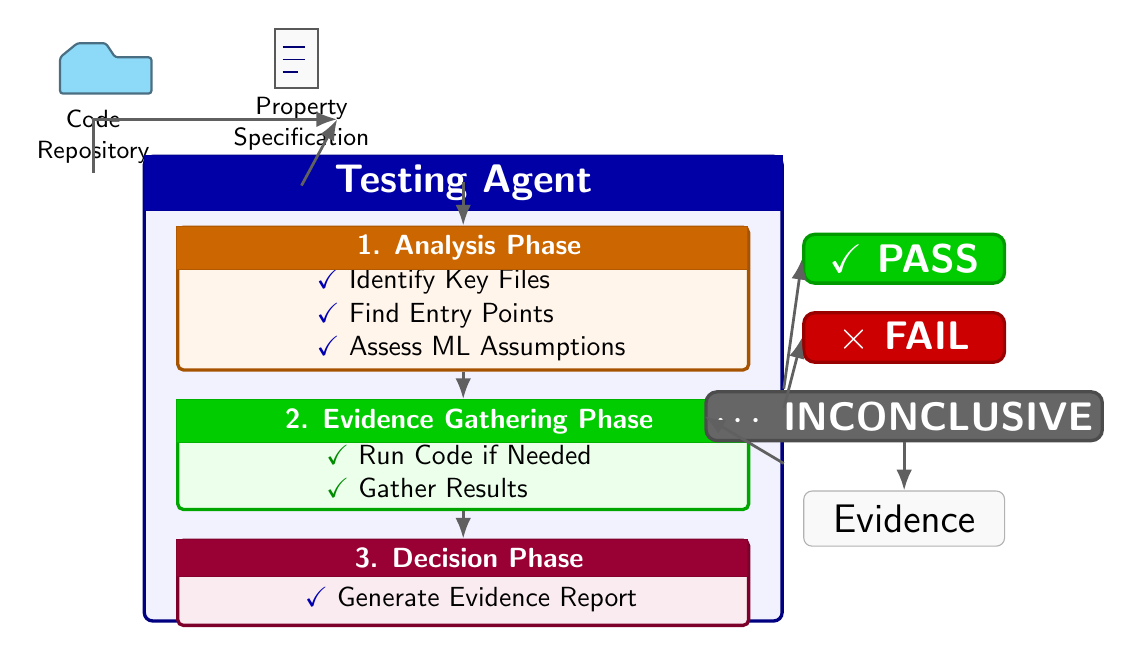
\begin{tikzpicture}[
    font=\sffamily,
    >=Latex,
    input/.style={align=center,font=\sffamily\small},
    box/.style={draw=blue!50!black,rounded corners=3pt,very thick,fill=blue!5,minimum width=8.1cm,minimum height=5.9cm},
    header/.style={draw=blue!60!black,fill=blue!65!black,text=white,font=\sffamily\bfseries\Large,minimum width=8.1cm,minimum height=0.7cm},
    phase/.style={draw=#1!65!black,rounded corners=2pt,very thick,fill=#1!8,minimum width=7.25cm,minimum height=1.38cm,align=left},
    phasehead/.style={draw=#1!70!black,fill=#1!80!black,text=white,font=\sffamily\bfseries,minimum width=7.25cm,minimum height=0.35cm,anchor=north west,align=left},
    verdict/.style={draw=#1!60!black,rounded corners=4pt,very thick,fill=#1!80!black,text=white,font=\sffamily\bfseries\Large,minimum width=2.55cm,minimum height=0.62cm,align=center},
    smallbox/.style={draw=gray!60,rounded corners=3pt,fill=gray!5,font=\sffamily\Large,minimum width=2.55cm,minimum height=0.7cm,align=center},
    flow/.style={->,line width=1pt,draw=gray!75!black}
  ]
    \node[input] (repo) at (-4.7,3.2) {Code\\Repository};
    \node[input,right=0.8cm of repo] (prop) {Property\\Specification\\in Markdown};
    \draw[fill=cyan!45!white,draw=cyan!45!black,thick,rounded corners=1pt]
      ([xshift=-0.42cm,yshift=0.55cm]repo.north) -- ++(0.22,0.18) -- ++(0.36,0) -- ++(0.12,-0.18) -- ++(0.46,0)
      -- ++(0,-0.46) -- ++(-1.16,0) -- cycle;
    \draw[fill=gray!5,draw=gray!70!black,thick]
      ([xshift=-0.34cm,yshift=0.75cm]prop.north) rectangle ++(0.55,-0.75);
    \draw[draw=blue!45!black,line width=0.5pt]
      ([xshift=-0.24cm,yshift=0.52cm]prop.north) -- ++(0.28,0)
      ([xshift=-0.24cm,yshift=0.36cm]prop.north) -- ++(0.28,0)
      ([xshift=-0.24cm,yshift=0.20cm]prop.north) -- ++(0.20,0);

    \node[box] (agent) at (0,0) {};
    \node[header,anchor=north] at (agent.north) {Testing Agent};

    \node[phase=orange,anchor=north] (analysis) at ([yshift=-0.9cm]agent.north) {
      \vspace{0.32cm}
      \hspace{0.2cm}\textcolor{blue!70!black}{\checkmark}\ Understand Repository\\
      \hspace{0.2cm}\textcolor{blue!70!black}{\checkmark}\ Identify Key Files\\
      \hspace{0.2cm}\textcolor{blue!70!black}{\checkmark}\ Find Entry Points\\
      \hspace{0.2cm}\textcolor{blue!70!black}{\checkmark}\ Assess ML Assumptions
    };
    \node[phasehead=orange] at (analysis.north west) {\hspace{0.18cm}1. Analysis Phase};

    \node[phase=green,anchor=north] (evidence) at ([yshift=-0.35cm]analysis.south) {
      \vspace{0.32cm}
      \hspace{0.2cm}\textcolor{green!55!black}{\checkmark}\ Review Code \& Tests\\
      \hspace{0.2cm}\textcolor{green!55!black}{\checkmark}\ Run Code if Needed\\
      \hspace{0.2cm}\textcolor{green!55!black}{\checkmark}\ Gather Results
    };
    \node[phasehead=green] at (evidence.north west) {\hspace{0.18cm}2. Evidence Gathering Phase};

    \node[phase=purple,minimum height=1.08cm,anchor=north] (decision) at ([yshift=-0.35cm]evidence.south) {
      \vspace{0.32cm}
      \hspace{0.2cm}\textcolor{blue!70!black}{\checkmark}\ Determine Outcome\\
      \hspace{0.2cm}\textcolor{blue!70!black}{\checkmark}\ Generate Evidence Report
    };
    \node[phasehead=purple] at (decision.north west) {\hspace{0.18cm}3. Decision Phase};

    \draw[flow] (repo.south) |- ([xshift=-1.6cm,yshift=0.45cm]agent.north);
    \draw[flow] (prop.south) -- ([xshift=-1.6cm,yshift=0.45cm]agent.north);
    \draw[flow] ([yshift=-0.35cm]agent.north) -- (analysis.north);
    \draw[flow] (analysis.south) -- (evidence.north);
    \draw[flow] (evidence.south) -- (decision.north);

    \node[verdict=green] (pass) at (5.6,1.65) {\checkmark\ PASS};
    \node[verdict=red] (fail) at (5.6,0.65) {$\times$\ FAIL};
    \node[verdict=gray] (inc) at (5.6,-0.35) {$\cdots$\ INCONCLUSIVE};
    \node[smallbox] (evout) at (5.6,-1.65) {Evidence};

    \draw[flow] (agent.east) -- (pass.west);
    \draw[flow] ([yshift=-0.25cm]agent.east) -- (fail.west);
    \draw[flow] ([yshift=-0.95cm]agent.east) -- (inc.west);
    \draw[flow] (inc.south) -- (evout.north);
  \end{tikzpicture}}
  \caption{Overview of Vibetest. A repository and natural-language property specification are given to a sandboxed testing agent, which analyzes the repository, gathers evidence, and returns a \textsc{pass}, \textsc{fail}, or \textsc{inconclusive} verdict with supporting evidence.}
  \label{fig:overview}
\end{figure*}

We summarize our contributions as follows.
\begin{itemize}
  \item We formulate evidence verifiability as a core requirement for LLM-agent audits of ML repositories against natural-language properties.
  \item We introduce Vibetest, an LLM-agent auditor that produces \textsc{pass}/\textsc{fail}/\textsc{inconclusive} decisions with evidence reports for ML-pipeline properties.
  \item We evaluate Vibetest on a controlled synthetic Kaggle benchmark with known injected bugs and on a real-world Kaggle audit with 380 manually annotated \textsc{fail} verdicts.
  \item We identify a unifying evidence rule: \textsc{fail} requires a present-and-violating operation; missing or unverifiable evidence should be \textsc{inconclusive}.
  \item We evaluate a post-hoc LLM evidence verifier and show that the current same-backbone verifier does not yet provide the desired low-false-positive filter, motivating verifier-specific designs.
\end{itemize}

\section{Natural-Language Specifications for ML Pipelines}
\label{sec:specs}

ML pipeline correctness is often specified informally.
Practitioners say that there should be no train-test leakage, evaluation should use the held-out split, augmentation should apply only to training data, and a model should beat a simple baseline.
These statements are precise enough for a human reviewer to investigate, but not directly executable as formal properties.

We define an informal ML-pipeline property as a natural-language statement about expected behavior or artifacts in a repository.
Given a repository $R$ and a property $p$, the goal is to output a decision
$y \in \{\textsc{pass}, \textsc{fail}, \textsc{inconclusive}\}$ and an evidence report $E$.
The evidence report should cite files, code regions, logs, outputs, or execution traces sufficient for a human to verify $y$.
This differs from classical program analysis, where a formal predicate $\phi$ is checked over possible traces.
Here, the property itself is an input in natural language, and the system must decide how to operationalize it.

\subsection{ML Pipeline Properties}

Our Kaggle audit suite contains 16 natural-language properties covering common ML-pipeline issues.
The properties include split hygiene, model-selection hygiene, parameter updates, preprocessing validity, augmentation scope, class-imbalance handling, path leakage, metric definitions, sanity-check experiments, dataloader shuffling, evaluation determinism, device consistency, secret leakage, and avoidable Python loops.
The full list is included in \Cref{app:properties}.

Several properties require observing a concrete operation.
For example, ``the model can overfit a single batch to near-zero loss'' requires either an existing tiny-batch experiment or a successful agent-run probe.
The absence of such an experiment should not be treated as a failure of the model.
This makes ML pipeline testing a useful setting for studying evidence sufficiency.

\subsection{Datasets}

We evaluate on two ML-pipeline datasets, summarized in \Cref{tab:datasets}.

\paragraph{Synthetic Kaggle.}
We construct a controlled benchmark by prompting GPT-5.2-codex to inject ML-pipeline bugs into clean Kaggle-style notebooks.
The benchmark contains 25 Titanic notebooks, 25 Disaster Tweets notebooks, and 25 Diabetic Retinopathy notebooks.
Each notebook is evaluated against 15 properties, yielding 1,125 notebook-property pairs.
The label files include the injected repository path, ground-truth property labels, and descriptions of the injected violations.

\paragraph{Real Kaggle.}
We collect 121 public Kaggle notebooks: 50 Titanic, 50 Disaster Tweets, and 21 Diabetic Retinopathy.
Each notebook is evaluated against 16 properties.
Because real notebooks do not have complete ground-truth bug labels, we evaluate the precision of emitted \textsc{fail} verdicts through manual evidence audit.

\begin{table}[t]
  \centering
  \small
  \caption{ML-pipeline datasets used in this paper.}
  \label{tab:datasets}
  \begin{tabular}{lrrr}
    \toprule
    Dataset & Notebooks & Properties & Pairs \\
    \midrule
    Synthetic Titanic & 25 & 15 & 375 \\
    Synthetic Tweets & 25 & 15 & 375 \\
    Synthetic Diabetic & 25 & 15 & 375 \\
    \midrule
    Real Titanic & 50 & 16 & 800 \\
    Real Tweets & 50 & 16 & 800 \\
    Real Diabetic & 21 & 16 & 336 \\
    \bottomrule
  \end{tabular}
\end{table}

\section{Vibetest and Evidence Verification}
\label{sec:method}

We propose an agentic testing system for evaluating natural-language ML properties over repositories.
The system has two components: a testing agent that produces a decision and evidence report, and a post-hoc verifier that scores whether a reported \textsc{fail} is supported by its evidence.

\subsection{Testing Agent}

Vibetest takes two inputs: a repository and a property specification written in natural language.
It operates in a sandboxed copy of the repository and may inspect files, search code, execute commands, run notebooks or scripts, and collect outputs.
The agent uses GPT-5-mini as its backbone in all experiments reported here.

\paragraph{Phase 1: Analysis.}
The agent first builds a high-level model of the repository.
It identifies relevant files, entry points, datasets, model definitions, preprocessing steps, and evaluation code.
This phase narrows the search space for the target property.

\paragraph{Phase 2: Evidence gathering.}
The agent gathers evidence for or against the property.
Evidence can include code snippets, execution logs, metrics, plots, or generated checks.
For ML repositories, this may involve inspecting notebook cells, running evaluation commands, or tracing data splits.

\paragraph{Phase 3: Decision.}
The agent outputs \textsc{pass}, \textsc{fail}, or \textsc{inconclusive}.
\textsc{Pass} means the cited evidence supports the property.
\textsc{Fail} means the cited evidence demonstrates a violation.
\textsc{Inconclusive} means the evidence is missing, ambiguous, or insufficient.

\subsection{Evidence Verifier}

The verifier is a post-hoc LLM judge over Vibetest's \textsc{fail} verdicts.
It receives the property prompt, the agent's reasoning, and the cited evidence.
It returns a structured score in $[0,1]$, where higher scores indicate stronger evidence that the \textsc{fail} is justified.
The verifier also returns a short rationale and an evidence assessment.

This design lets us turn evidence sufficiency into a measurable prediction problem.
By thresholding verifier scores, we can accept only high-confidence failures and plot precision-recall tradeoff curves.
The desired verifier has a very low false-positive rate: it should rarely accept a \textsc{fail} whose evidence actually supports \textsc{inconclusive}.

\subsection{Evidence Rubric}
\label{sec:rubric}

We use a strict three-way rubric.
\begin{itemize}
  \item \textbf{\textsc{fail}}: the evidence demonstrates that a relevant operation is present and violates the property.
  \item \textbf{\textsc{pass}}: the evidence demonstrates that a relevant operation is present and satisfies the property.
  \item \textbf{\textsc{inconclusive}}: the operation is absent, cannot be inspected, cannot be executed, or is present but unverifiable.
\end{itemize}

The critical rule is that missing evidence is not negative evidence.
If the notebook does not run an experiment required by a property, the auditor has not shown that the experiment failed.
It has shown that the current evidence is insufficient.

\section{Experiments}
\label{sec:experiments}

\subsection{Setup}

We evaluate three questions.
First, how accurately does Vibetest detect injected ML-pipeline bugs in a controlled setting?
Second, how often are Vibetest's real-world \textsc{fail} verdicts supported by evidence?
Third, can a post-hoc LLM verifier reject unsupported \textsc{fail}s while preserving supported ones?

For the synthetic benchmark, we compute precision, recall, and F1 over notebook-property pairs using ground-truth injected bug labels.
For the real Kaggle setting, we manually audit \textsc{fail} verdicts because complete recall ground truth is unavailable.
The full real-world audit labels all 380 emitted \textsc{fail}s as Correct or Incorrect.
To address label-source overlap from LLM-assisted annotation, we also conduct a stricter 100-case re-audit.
The original audit used GPT-5.1 Thinking for code navigation and summarization; the re-audit restricts the assistant to retrieval and summary and applies the rubric in \Cref{sec:rubric}.

\subsection{RQ1: Can Vibetest Detect Synthetic ML Bugs?}

\Cref{tab:synthetic-results} reports Vibetest performance on the synthetic benchmark using evidence-verified ground truth matching.
Across 1,125 notebook-property pairs, Vibetest emits 476 \textsc{fail} predictions.
Of these, 280 correspond to ground-truth injected violations with supporting evidence, giving 58.8\% precision and 55.6\% recall.

\begin{table}[t]
  \centering
  \small
  \caption{Vibetest on synthetic Kaggle notebooks with injected bugs.}
  \label{tab:synthetic-results}
  \begin{tabular}{lrrrrr}
    \toprule
    Setting & Pairs & GT Fail & Pred Fail & Precision & Recall \\
    \midrule
    Synthetic Kaggle & 1,125 & 504 & 476 & 58.8 & 55.6 \\
    \bottomrule
  \end{tabular}
\end{table}

Vibetest recovers many injected bugs, but its false-positive rate is high enough that raw \textsc{fail}s are not yet reliable without further verification.
This motivates evidence-level evaluation rather than reporting classification alone.

\subsection{RQ2: Are Real-World Failures Supported by Evidence?}

On 121 real Kaggle notebooks, Vibetest emits 380 \textsc{fail} verdicts.
The full manual audit labels 251 as Correct and 129 as Incorrect, giving 66.1\% precision.
However, the stricter 100-case re-audit reveals that the original labels are permissive.
Within the re-audited sample, 64 cases are Correct under the original labels, but only 40 remain valid \textsc{fail}s under the present-and-violating rubric.
The remaining cases become \textsc{inconclusive} or \textsc{pass}.

\begin{table}[t]
  \centering
  \small
  \caption{Evidence audit of real Kaggle \textsc{fail} verdicts.}
  \label{tab:real-audit}
  \begin{tabular}{lrrrr}
    \toprule
    Audit & Cases & Valid & Invalid & Precision \\
    \midrule
    Full original audit & 380 & 251 & 129 & 66.1 \\
    100-case original labels & 100 & 64 & 36 & 64.0 \\
    100-case strict re-audit & 100 & 40 & 60 & 40.0 \\
    \bottomrule
  \end{tabular}
\end{table}

The difference between the original audit and the strict re-audit is central to the paper.
Many apparent failures are better understood as failures to obtain evidence.
This is especially visible for tests that require an experiment.
Across the 121 real notebooks, randomized-label sanity receives 0 \textsc{pass}, 44 \textsc{fail}, and 77 \textsc{inconclusive} verdicts.
Baseline comparison receives 0/23/98, training-loss behavior receives 0/7/114, and tiny-batch overfit receives 1/13/107.
Among 22 experiment-required \textsc{fail}s in the strict re-audit sample, 21 become \textsc{inconclusive}.

\subsection{RQ3: Can a Post-Hoc Verifier Filter Bad Evidence?}

We evaluate the LLM verifier as a filter over \textsc{fail} verdicts.
The intended use is to accept only \textsc{fail}s whose verifier score exceeds a threshold $\tau$, thereby trading recall for higher precision.
In the current same-backbone run, this does not yet work.
On synthetic predicted \textsc{fail}s, verifier AUROC is approximately 0.50.
On the 100-case real sample, AUROC is 0.47 against the original labels and 0.42 against the strict re-audit.
At $\tau = 0.7$, the verifier accepts 22 strict re-audit cases, only 8 of which are valid \textsc{fail}s.

\begin{table}[t]
  \centering
  \small
  \caption{Current post-hoc evidence-verifier results. Base precision is the precision before verifier filtering.}
  \label{tab:verifier}
  \begin{tabular}{lrrrr}
    \toprule
    Labels & Cases & Base P & AUROC & P @ .7 \\
    \midrule
    Synthetic predicted \textsc{fail}s & 476 & 58.8 & 0.50 & 71.8 \\
    Real original labels & 100 & 64.0 & 0.47 & 59.1 \\
    Real strict re-audit & 100 & 40.0 & 0.42 & 36.4 \\
    \bottomrule
  \end{tabular}
\end{table}

This result suggests that simply asking another GPT-5-mini-based model to judge evidence is not enough.
The verifier often shares the same permissive interpretation as the original auditor.
Future verifier designs should be evaluated by the low-false-positive criterion: the verifier should rarely accept a failure unless it can identify the present operation and the violation.

\section{Analysis: The Underlying Evidence Error}

Incorrect \textsc{fail}s fall into several surface categories, but they share one rule violation.

\paragraph{Absence-as-failure.}
The agent reports a failure because it cannot find evidence that a property is satisfied.
For example, it may fail a randomized-label sanity test because no such experiment is present.

\paragraph{Best-practices-as-requirements.}
The agent treats missing recommended practice as a correctness violation.
Not every Kaggle notebook runs tiny-batch overfitting or baseline comparisons, but absence of these checks is not itself a failed check.

\paragraph{Notebook over-interpretation.}
The agent sometimes treats partial, stale, or exploratory notebook cells as if they define the complete training pipeline.
This is common in Kaggle notebooks where cells may be run out of order or left as abandoned experiments.

\paragraph{Missing-output-as-incorrect-output.}
The agent treats absent logs or plots as evidence of incorrect behavior.
For example, no training-loss curve does not imply that training loss failed to decrease.

These categories motivate a single operational rule for agentic audits:
\textsc{fail} should require evidence of a present-and-violating operation.
If the relevant operation is absent or unverifiable, the agent should return \textsc{inconclusive}.

\section{Related Work}

\paragraph{LLM agents for repository auditing.}
RepoAudit \citep{guo2025repoaudit} and BugScope \citep{liu2025bugscope} study LLM-based repository-level bug detection.
SWE-bench \citep{jimenez2024swebench} and related agentic software-engineering benchmarks evaluate repository-scale issue resolution.
Our work focuses on a complementary problem: verifying the evidence behind natural-language audit verdicts in ML pipelines.

\paragraph{ML pipeline correctness.}
ML debugging and monitoring tools such as Model Assertions \citep{kang2020assertions}, TorchQL \citep{naik2024torchql}, UMLAUT \citep{schoop2021umlaut}, and DEFault \citep{wang2025default} target correctness properties in ML systems.
These methods usually require formalized checks, query languages, or expert-defined rules.
Vibetest instead accepts natural-language properties and studies how reliably an LLM agent can operationalize them.

\paragraph{LLM verifiers and judges.}
LLM verifiers have improved reasoning by separating generation from checking \citep{cobbe2021verifier,lightman2024process}.
LLM-as-judge methods evaluate open-ended outputs \citep{zheng2023judge,tan2025judgebench}, and self-verification methods ask models to check their own reasoning \citep{weng2023selfverification}.
Our verifier judges whether code-audit evidence supports a \textsc{fail} verdict.
The current negative result highlights the need to evaluate verifier independence rather than assuming a second LLM call provides reliable validation.

\paragraph{Natural-language task specifications.}
Instruction following is a core NLP problem \citep{ouyang2022instruct,zhou2023instruction,sclar2024prompt}.
Natural-language code audits are a particularly demanding setting because the specification is short, the repository context is large, and the output has operational consequences.
Our results show that the boundary between \textsc{fail} and \textsc{inconclusive} is a key specification-following challenge.

\section{Conclusion}

We studied evidence-based verification for LLM-agent audits of ML pipelines.
Vibetest can find many injected and real ML-pipeline issues from natural-language properties, but many of its \textsc{fail} verdicts are not supported by sufficiently strong evidence.
The dominant error is structural: the agent treats missing evidence as evidence of violation.
We formalize a stricter present-and-violating rubric and evaluate a post-hoc LLM verifier intended to filter unsupported failures.
The current same-backbone verifier is not yet reliable, but this negative result clarifies the path forward.
For natural-language code auditors to be useful, verdict generation and evidence verification must be separated, measured, and optimized directly.

\section*{Limitations}

\paragraph{Single annotator.}
The full 380-case real-world audit was labeled by one annotator.
We mitigate this with a 100-case strict re-audit but do not report inter-annotator agreement.

\paragraph{LLM-assisted annotation.}
The original audit used GPT-5.1 Thinking for code navigation and summarization.
This creates potential label-source overlap with LLM verifier evaluation.
The strict re-audit was designed to reduce this overlap and is reported separately.

\paragraph{Single verifier backbone.}
The current verifier uses GPT-5-mini, the same backbone family as Vibetest.
We do not yet evaluate cross-backbone verification, verifier-specific training, or calibrated verifier prompts.

\paragraph{Real-world recall.}
The real-world Kaggle setting has no complete bug ground truth.
We audit precision of emitted \textsc{fail}s but cannot measure recall on real notebooks.

\paragraph{Kaggle notebook style.}
Kaggle notebooks are exploratory and sometimes incomplete.
The notebook over-interpretation failure mode may be less common in production ML repositories with clearer entry points and test harnesses.

\section*{Ethical Considerations}

\paragraph{Deployment risk.}
Unsupported automated bug reports can waste developer time and erode trust in code-auditing tools.
Our results argue against deploying LLM-agent auditors as replacements for human review.
They should be used as assistive systems with inspectable evidence and calibrated uncertainty.

\paragraph{Data provenance.}
The real-world audit uses public Kaggle notebooks.
We do not redistribute notebook contents in the paper.
Supplementary material should reference notebooks by public identifiers and include derived annotations only where licensing permits.

\paragraph{Use of AI assistance.}
The system under study is an LLM-agent auditor backed by GPT-5-mini.
GPT-5.1 Thinking was used as an assistant during the original manual audit for code navigation and summarization, with final labels assigned by the human annotator.
GPT-5.2-codex was used to construct the synthetic injected-bug benchmark.
This draft was prepared with AI writing assistance and should be disclosed according to the ACL Policy on AI Writing Assistance.

\bibliographystyle{acl_natbib}
\bibliography{vibetest}

\appendix

\section{Full ML Pipeline Property List}
\label{app:properties}

\begin{itemize}
  \item No leakage from test to train/val sets.
  \item If there is any model selection or hyperparameter tuning, then it uses val only.
  \item If there is any model training, then all model parameters are updated during training (no frozen layers unless explicitly intended).
  \item Data is loaded and preprocessed correctly (e.g., no all-black images, no text with weird or unexpected characters, tables look correct and feature values are reasonable).
  \item Any data augmentation is only performed on the training dataset; val/test dataset use deterministic preprocessing.
  \item Any class-imbalance handling (weighted loss / sampler) applies only to training data.
  \item No path/filename text is fed as a feature unless explicitly intended.
  \item Reported metrics use the correct split(s) and the exact definitions claimed (e.g., micro vs macro, top-k).
  \item Randomizing the labels results in accuracy dropping to be near a random guessing baseline (may not be 0.5 if the data is imbalanced) on a validation set.
  \item The model after the full training procedure outperforms a simple baseline (e.g., random or majority class) on an evaluation set.
  \item The model can overfit a single (or tiny) batch to near-zero loss.
  \item Training loss generally decreases during training and plateaus within the number of epochs used (if no loss is logged, then add logging to check this).
  \item Training dataloader shuffles or training dataset is shuffled for training; val/test do not shuffle.
  \item Accuracy should be deterministic (same value) when running the model evaluation multiple times without retraining.
  \item Model and inputs are consistently moved to one device; no implicit CPU-to-GPU transfers; dtype policy (e.g., fp32/bf16) is applied consistently.
  \item Code does not include any secrets (API keys, passwords, etc.).
  \item Code does not use explicit loops or Python control flow when matrix operations could have been used to implement the exact same operation more efficiently.
\end{itemize}

\end{document}
